\documentclass{beamer}
%
% Choose how your presentation looks.
%
% For more themes, color themes and font themes, see:
% http://deic.uab.es/~iblanes/beamer_gallery/index_by_theme.html
%
\mode<presentation>
{
  \usetheme{Madrid}      % or try Darmstadt, Madrid, Warsaw, ...
  \usecolortheme{default} % or try albatross, beaver, crane, ...
  \usefonttheme{default}  % or try serif, structurebold, ...
  \setbeamertemplate{navigation symbols}{}
  \setbeamertemplate{caption}[numbered]
} 

\usepackage[english]{babel}
\usepackage[utf8x]{inputenc}
\usepackage{bm}

\title[]{Spatial-temporal Modeling of Ambient Ozone}
\author{Lucy Lu, Sam Yin}
\institute{DSS, Duke University}
\date{May 2, 2017}

\begin{document}

\begin{frame}
  \titlepage
\end{frame}

\begin{frame}{Outline}
  \tableofcontents
\end{frame}

\section{Data}

\begin{frame}{Introduction}
\begin{itemize}
\item Ground level ozone (ppb) 
\item Collected at 1249 sites in the U.S. from 06/01/2015 00:00:00 to 06/30/2015 23:00:00 at hourly frequency. 
\end{itemize}
\begin{figure}
\centering
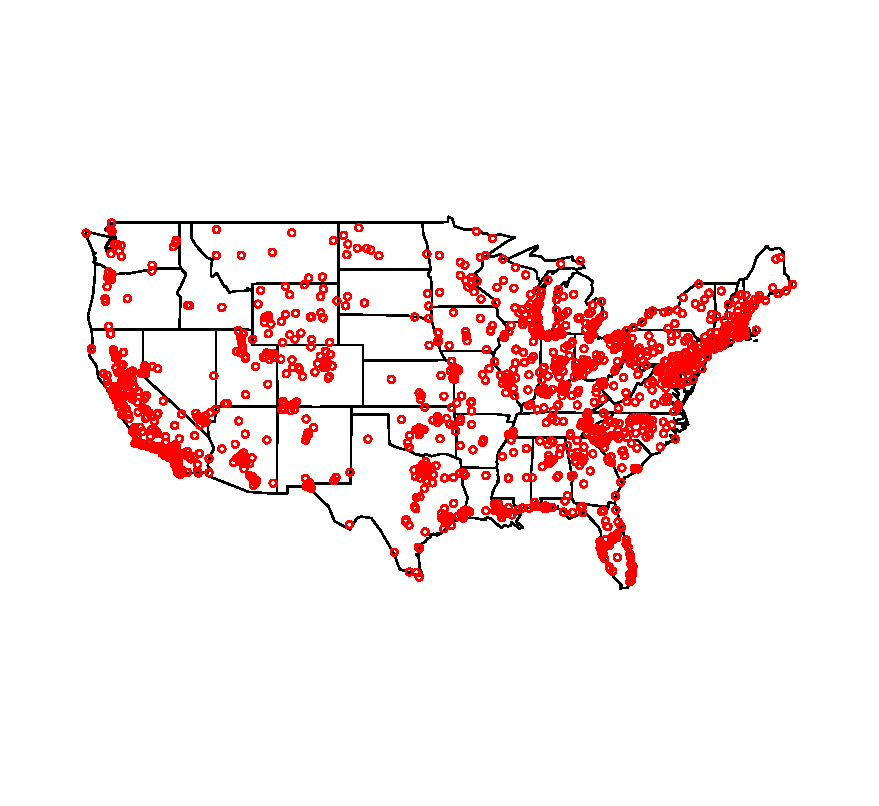
\includegraphics[scale = 0.35]{site_map.eps}
\caption{Map of ozone sites across the U.S.}
\end{figure}
\end{frame}

\begin{frame}{Data Preprocessing}
\begin{itemize}
\item Keep sites where data completeness is at least 95\%
\item Divide the U.S. into 25 subregions and model by region
\item Impute missing values by averaging the two closest available observations along the temporal dimension
\end{itemize}
\begin{figure}
\centering
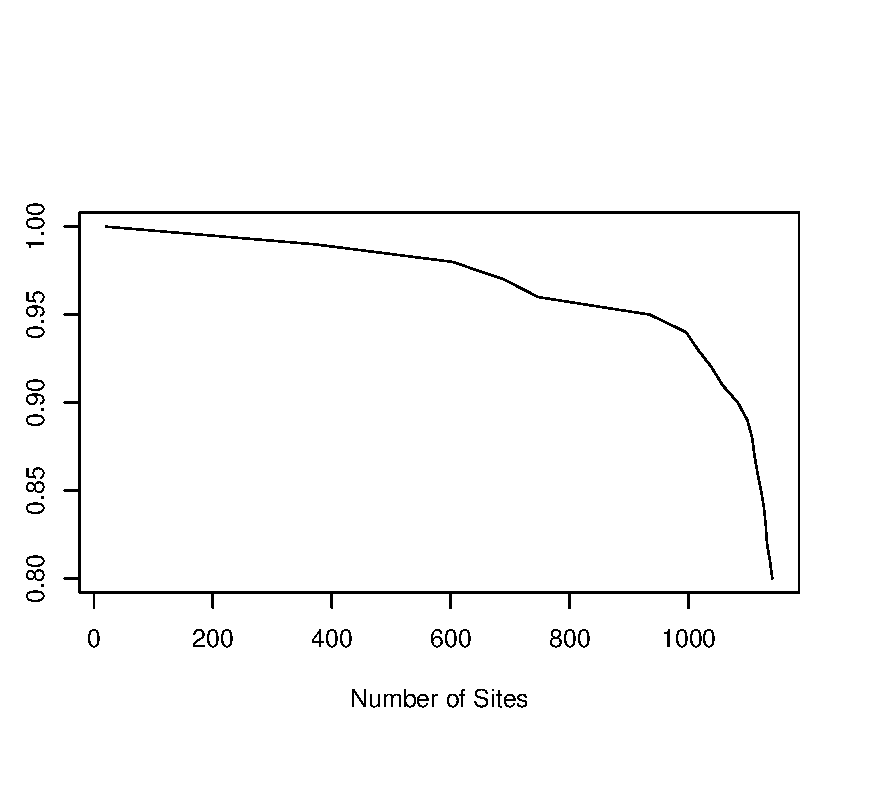
\includegraphics[scale = 0.3]{completeness_by_n_sites.eps}
\caption{Cut-off percentage of completeness by number of sites}
\end{figure}
\end{frame}

\begin{frame}{EDA}
\begin{figure}
\centering
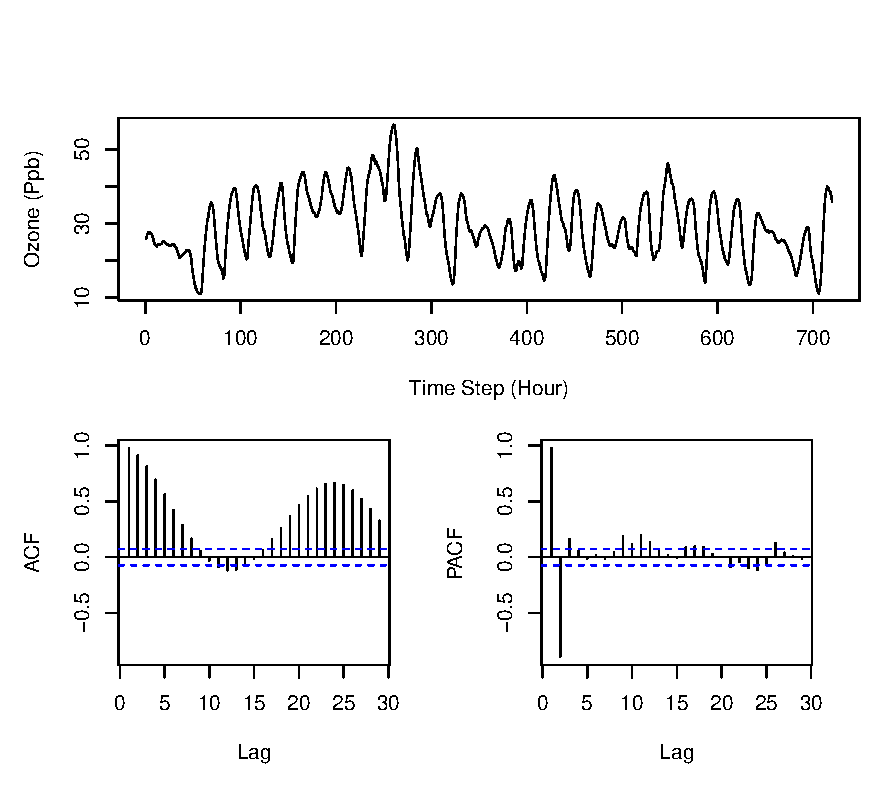
\includegraphics[scale = 0.4]{ts_o3.eps}
\caption{Time series display of average ozone (of all sites) in region 1}
\end{figure}
\end{frame}

\begin{frame}{EDA (cont.)}
\begin{figure}
\centering
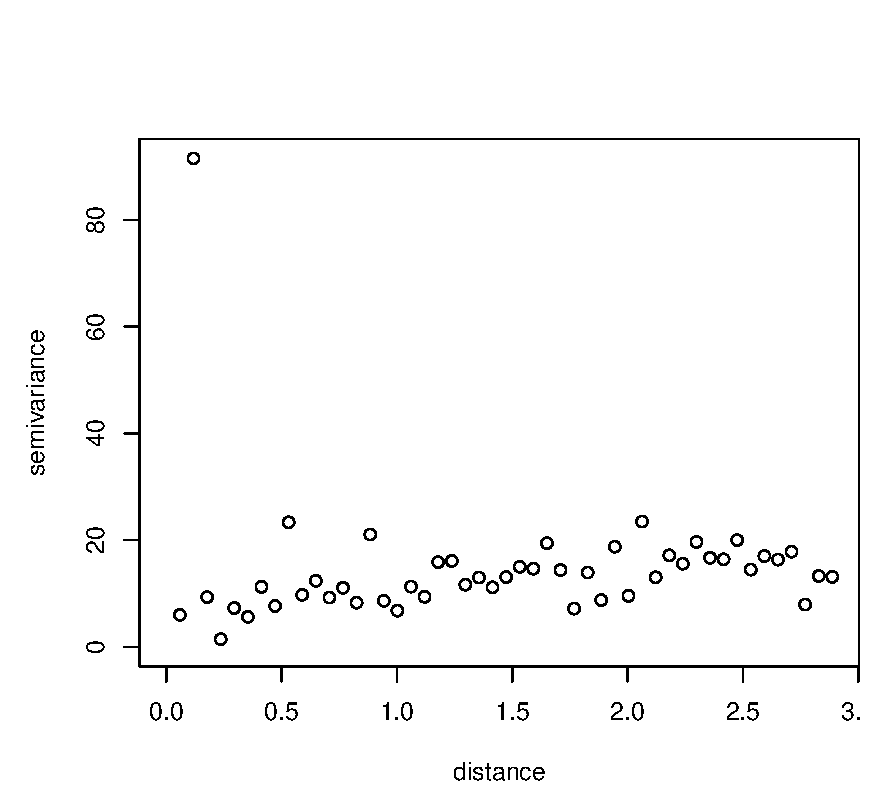
\includegraphics[scale = 0.4]{variogram.eps}
\caption{Variogram of average ozone (of all time steps) in region 1}
\end{figure}
\end{frame}

\section{Modeling Ideas}

\begin{frame}{Modeling Ideas}
Assuming no dependence between spatial and temporal dimensions, we build models with the additive structure (2). In other words, $\alpha(t)$ is constant to all sites at a given time point, and $\omega(s)$ is constant at all time points given a specific site.
\begin{align}
y(s, t) &= w(s, t) + e(s, t) \\
&= \alpha(t) + \omega(s) + \epsilon(s, t)
\end{align}
\end{frame}

\begin{frame}{Modeling Ideas (cont.)}
Temporal specification:
\begin{enumerate}
\item AR(1): $\alpha(t) = \delta + \phi \alpha(t - 1)$ 
\item MA(1): $\alpha(t) = \delta + w_t + \theta w_{t - 1},\ w_{1:T} \overset{\text{i.i.d.}}{\sim} N(0, \sigma_w^2)$
\end{enumerate}

Spatial specification: 
\begin{equation}
\omega(\tilde{s}) \sim \mbox{MVN}(\mathbf{0}, \bm{\Sigma}_{\omega})
\end{equation}
where $\{\Sigma_{\omega}\}_{ij} = \sigma_\omega^2 \exp(-\phi_{\omega}||s_i - s_j||_2)$ for $i \neq j$ \\
Error specification: \\
\begin{equation}
\epsilon(s, t) \sim N(0, \sigma_\epsilon^2)
\end{equation}
\end{frame}

\begin{frame}{Model Fitting}
\begin{itemize}
\item Use a 120-hour learning window for every next-hour ozone forecast
\item Use 47 sites for model training and 24 sites for kriging
\item JAGS, 4000 iterations, 3000 burn-ins, 3 chains
\item First make next-hour forecasts at observed sites, then krige to unobserved sites by sampling from conditional multivariate normal distribution with covariance specified by GP
\end{itemize}
\end{frame}

\begin{frame}{Evaluation Criteria}
\begin{align*}
\text{PMSE} &= \frac{\sum_{t = 1}^m\sum_{s = 1}^{n}(\hat{y}(s, t) - y_{obs}(s, t))^2}{mn} \\
\text{Average Interval Length} &= \frac{\sum_{t = 1}^{m}\sum_{s = 1}^{n}\text{Length of 95\% CI at Time $t$ Site $s$}}{mn} \\
\text{Coverage} &= \frac{\sum_{t = 1}^{m}\sum_{s = 1}^{n}\mathbf{1}(y_{obs}(s, t) \in 95\% CI)}{mn} \\
\text{CRPS} &= E_{F}|y(s, t) - y_{obs}(s, t)| - \frac{1}{2}E_{F}|y(s, t) - y'(s, t)|
\end{align*}
\end{frame}

\section{Results}

\begin{frame}{Results}
\begin{table}[H]
\centering
\begin{tabular}{|c c c c c|}
\hline
Model & PMSE & Interval & Coverage & CRPS \\\hline 
AR(1) & 17.7 & 12.98 & 0.85 & 2.36\\
MA(1) & 126.24 & 36.56 & 0.91 & 6.56 \\\hline
\end{tabular}
\caption{Summary of predictive performance at fitting sites (47)}
\end{table}

\begin{table}[H]
\centering
\begin{tabular}{|c c c c c|}
\hline
Model & PMSE & Interval & Coverage & CRPS \\\hline 
AR(1) & 60.08 & 12.84 & 0.79 & 4.29\\
MA(1) & 38.00 & 27.49 & 0.92 & 3.45 \\\hline
\end{tabular}
\caption{Summary of predictive performance at kriging sites (24)}
\end{table}
\end{frame}

\begin{frame}{Results (cont.)}
\begin{table}[H]
\centering
\begin{tabular}{|c c c|c c c|}
\hline
AR(1) & Mean & 95\% CI & MA(1) & Mean & 95\% CI \\\hline
$\sigma_\omega^2$ & 4.32 & (3.59, 5.20) & $\sigma_\omega^2$ & 49.97 & (44.95, 55.55) \\
$\phi_\omega$ & 0.15 & (0.10, 0.20) & $\phi_\omega$ & 0.57 & (0.48, 0.67) \\
\hline
$\phi$ & 0.88 & (0.87, 0.89) & $\theta$ & 1.06 & (0.76, 1.44) \\
$\delta$ & 3.83 & (2.80, 5.14) & $\sigma_w^2$ & 13.26 & (7.76, 20.21) \\
$\sigma_\epsilon^2$ & 6.40 & (6.07, 6.75) & $\delta$ & 25.51 & (24.11, 26.94) \\
 &  &  & $\sigma_\epsilon^2$ & 14.68 & (13.00, 16.41) \\
\hline
\end{tabular}
\caption{Summary of parameter posterior distributions}
\end{table}
\end{frame}

\begin{frame}{Results (cont.)}
\begin{figure}
\centering
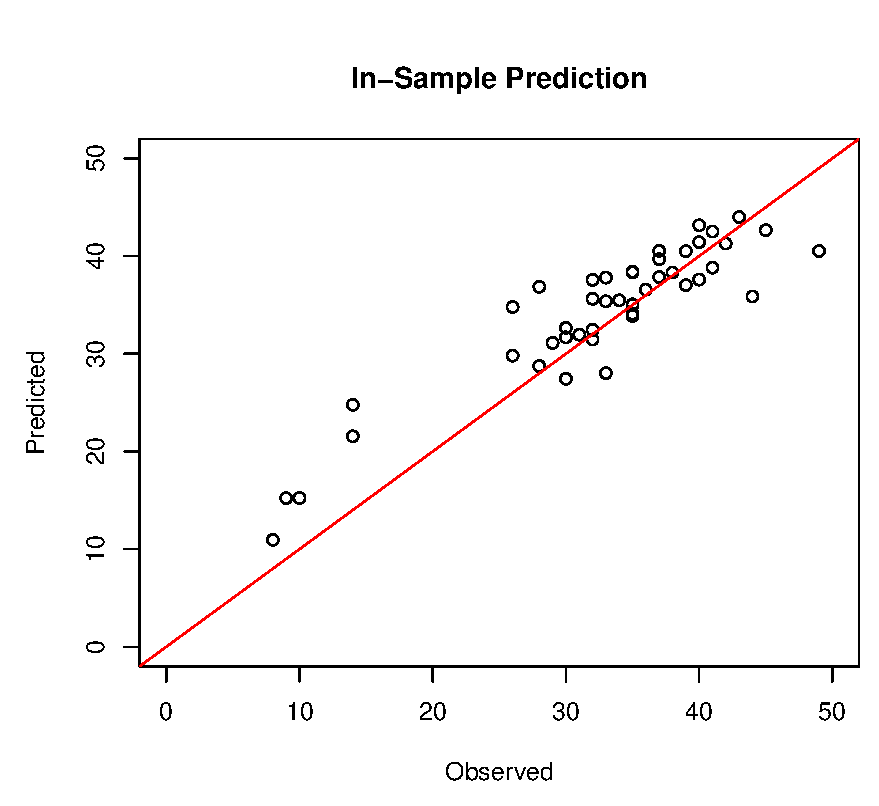
\includegraphics[scale = 0.35]{pred_in_ar.eps}
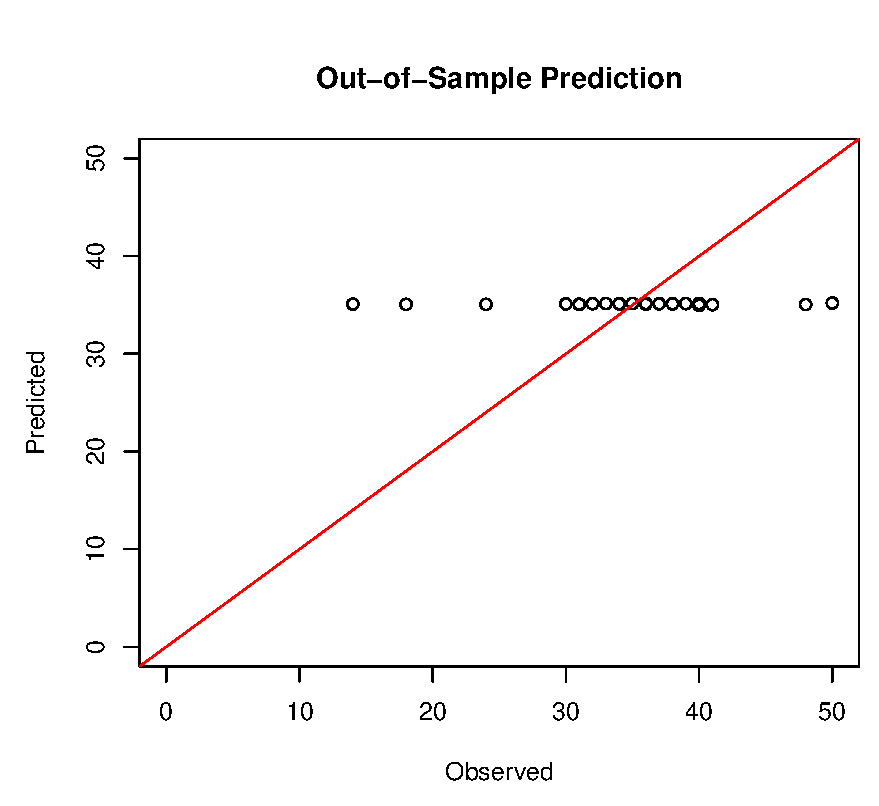
\includegraphics[scale = 0.35]{pred_out_ar.eps}
\caption{Pedicted vs observed ozones, AR(1)}
\end{figure}
\end{frame}

\begin{frame}{Results (cont.)}
\begin{figure}
\centering
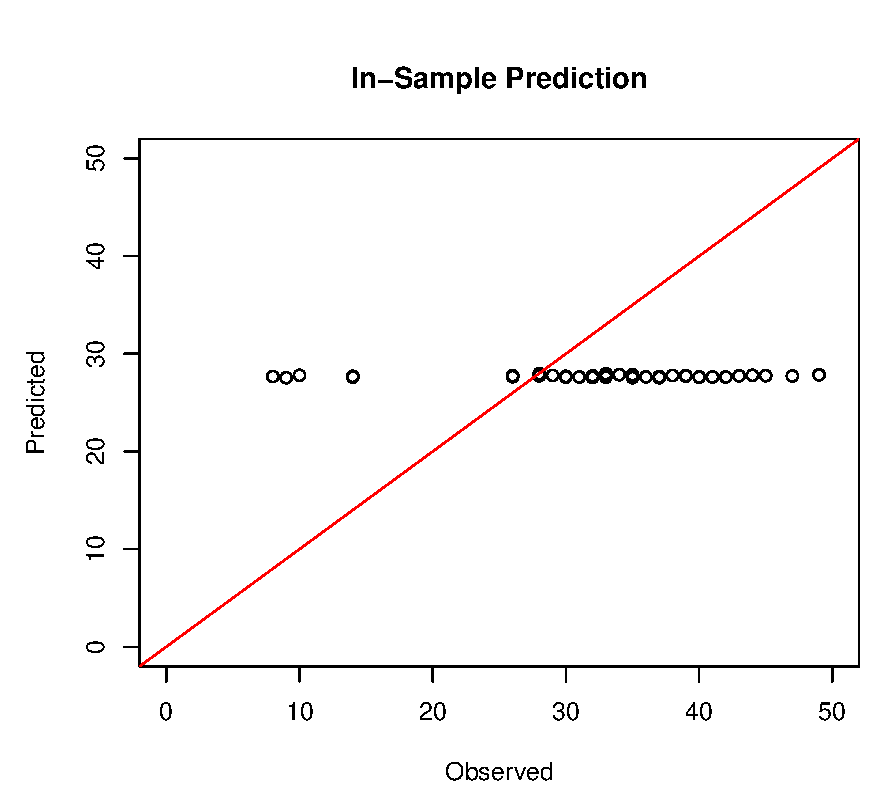
\includegraphics[scale = 0.35]{pred_in_ma.eps}
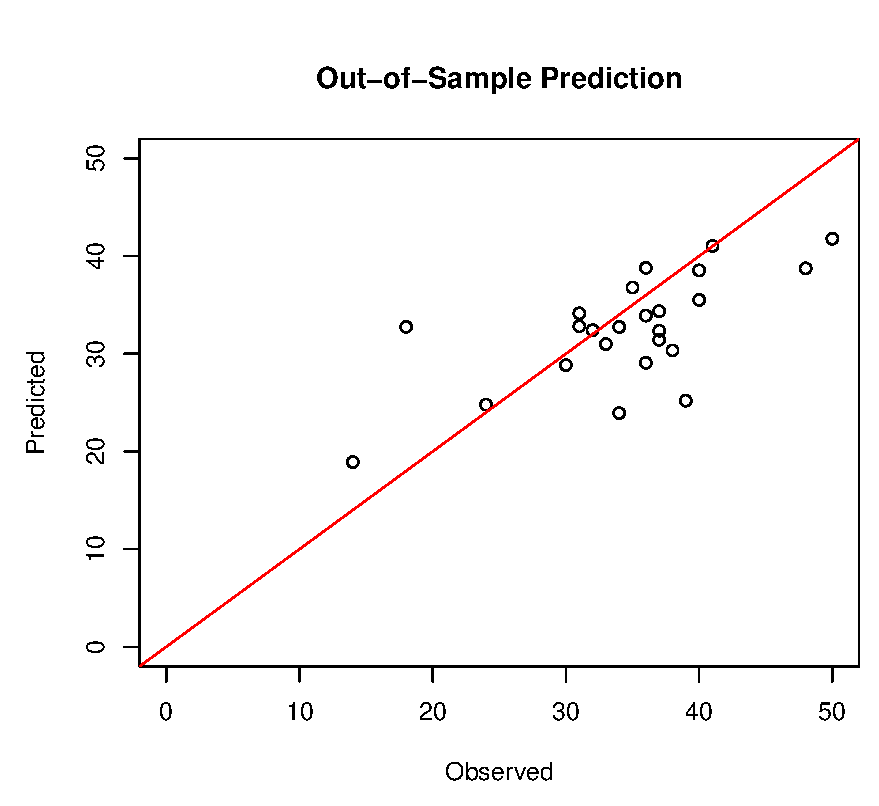
\includegraphics[scale = 0.35]{pred_out_ma.eps}
\caption{Pedicted vs observed ozones, MA(1)}
\end{figure}
\end{frame}


\section{Discussion}

\begin{frame}{Discussion}
\begin{itemize}
	\item In-sample vs. Out-of-sample (kriging) prediction
    \item Time series
    \item Additive assumption \& Computational efficiency
\end{itemize}
\end{frame}

\end{document}
